\chapter{An Introduction to BeagleSNES}

\section{Overview}\index{Overview}

BeagleSNES is a complete software system that turns the ARM-based BeagleBoard-xM (BB-xM) and BeagleBone Black (BBB) hardware platforms\footnote{Learn more about the BeagleBoard family of hardware platforms at \texttt{www.beagleboard.org}.} into a dedicated device capable of executing software that was originally developed for the Super Nintendo Entertainment System\textregistered  (SNES) video game console\footnote{Nintendo\textregistered and Super Nintendo Entertainment System\textregistered are registered trademarks of Nintendo Co. Ltd. and its subsidiary companies.}.  It allows you to play SNES titles on your television or computer monitor via the DVI digital video output of the BB-xM and the HDMI output of the BBB. The BBB also supports using the LCD3 cape for video output. 

\begin{figure}[h]
\centering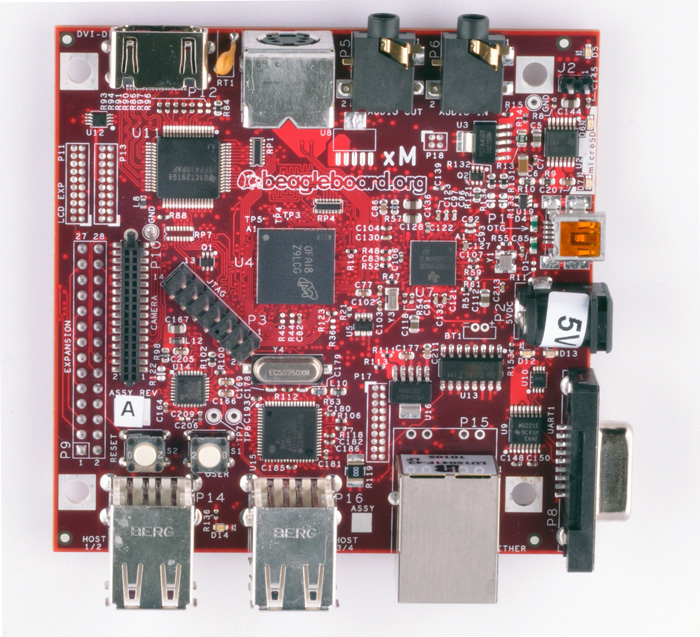
\includegraphics[scale=0.3]{intro_chapter/beagleboard_xm2.jpg} 
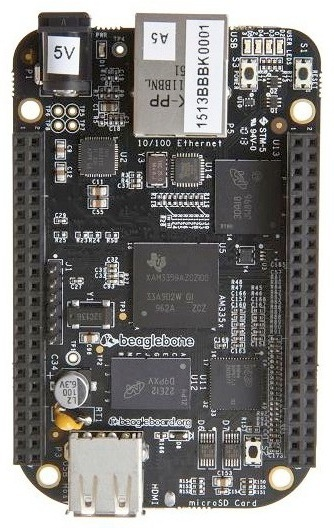
\includegraphics[scale=0.35]{intro_chapter/beagleboardblack.jpg} 
\caption{The BeagleBoard-xM (left) and BeagleBone Black (right) hardware platforms.}
\end{figure}

BeagleSNES originally began as a course project for a graduate embedded systems design class.  While the scope of the project was to port the SNES9X emulator to the BB-xM and then tune the board's Linux kernel for performance, things got a little out of hand.  The project kept growing in complexity and scope.  Over the span of four months, it matured into the initial release of the project that you see today.  The bootloader, Linux kernel, file system, and emulator of BeagleSNES have all been customized for functionality, stability, and performance.  These components were further customized when the project was ported to the BBB.

The source code for BeagleSNES, as well as the latest instructions for building, installing, and using the software, are freely available from \texttt{www.beaglesnes.org}.  Almost all of BeagleSNES is licensed under the GNU Public License (version 3) as open source software (OSS), but the emulator itself is licensed under a custom, non-commercial license.  What does this mean?  It means that you are welcome to examine the code, modify it, learn from it, and even use it in projects of your own.  But, you may not sell the system if it contains the emulator. 

The hardware of the SNES (CPU, GPU, memory, audio chipset, etc.) is quite different from the hardware of the BB-xM and BBB.  SNES software will never execute natively on these platforms, so BeagleSNES must \emph{emulate} the hardware of the SNES in software.  The inputs, outputs, and internal state of each piece of SNES hardware is represented as high-level source code (C and C++ code, in the case of BeagleSNES).  The 16-bit microprocessor of the SNES (the WDC 65C816) runs at a clock speed of 3.58 MHz.  This is much slower than the 32-bit ARM CPUs of the BB-xM (AM37x 800 MHz Cortex-A8) and BBB (AM335x 1 GHz Cortex-A8), meaning that there are enough resources available to dynamically translate every SNES program instruction, at the time that it would be executed on the SNES, into one or more ARM instructions and then execute them.  This \emph{just-in-time dynamic translation} approach has considerable overhead, but it is very effective in situations where the emulated system is much slower than the system performing the emulation.

\begin{figure}[h]
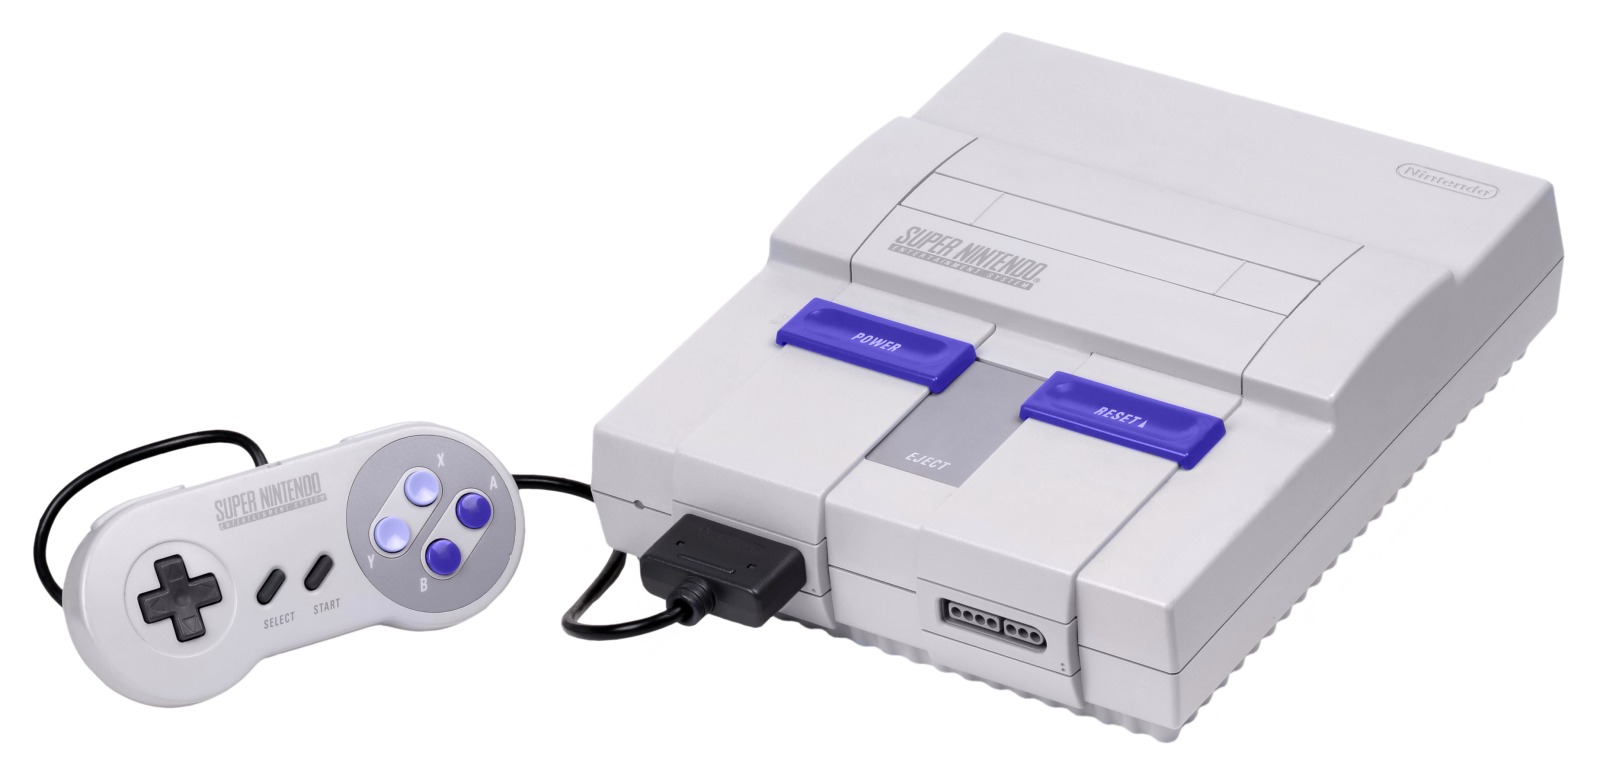
\includegraphics[scale=0.25]{intro_chapter/Super_Nintendo_North_America_Model.png}
\caption{The Super Nintendo Entertainment System\textregistered video game console.}
\end{figure}

Several SNES emulators currently exist, and BeagleSNES leverages this existing work (rather than "reinventing the wheel").  The SNES9X emulator\footnote{www.snes9x.com} was selected to serve as the emulator base for the project for the following reasons:

\begin{itemize}
\item All source code for the emulator is available, and all optimizations and additions made to it as part of BeagleSNES can be freely released as long as the terms of the SNES9X license are followed.
\item The source code for the emulator is cross-platform, meaning that its implementation is not tied to a particular display library or CPU architecture.
\item Its emulation compatibility is quite good, allowing it to run many different pieces of SNES software accurately.
\end{itemize}

While many architecture-specific performance optimizations exist in SNES9X (such as using x86-based assembly cores to accelerate the emulation), many of these improvements can't be used with the ARM-based BB-xM and BBB.  This limits the overall emulation speed of BeagleSNES, but the performance is generally acceptable.  

\section{Using This Manual}\index{Using This Manual}

This guide was written to help you to install and configure BeagleSNES.  It also contains technical information that provides details of how the system works and describes how to build the various components of the system from source.  Hopefully, this information will not only allow you to enjoy BeagleSNES for your own entertainment, but also allow you to use this work as a basis for whatever BeagleBoard-based system you might want to create.  

For any important aspects of the system that warrant additional attention, this manual uses the following box to highlight them:

\begin{updateWarn}
Be sure to pay attention to these boxes as you read through the manual.  They will alert you to any important or useful information that you should be aware of.
\end{updateWarn}

For any commands executed on the command line, this manual uses the following box:

\begin{commandBox}
\texttt{username@host\$  sudo ./execute\_this\_command}
\end{commandBox}

Each section of the guide contains information on a different aspect of BeagleSNES.  Section 1 is the introduction that you are reading right now.  Section 2 describes how to download and install the pre-made file system image of BeagleSNES.  For most end-users, this section will be the most important one to review.  Section 3 provides instructions on how to add ROMs to the BeagleSNES system and configure the game selection GUI and gamepad button mapping.  Section 4 is a troubleshooting guide to help you work through some of the common issues that people come across.  Section 5 gives step-by-step instructions on how to build the various pieces of the BeagleSNES system.  Section 6 provides more details about the configuration of the bootloader and Linux kernel used in BeagleSNES.  Section 7 describes several details of the audio, video, and input subsystems of BeagleSNES.  This will be of interest to developers that wish to review the technical details of how BeagleSNES interfaces with the BeagleBoard hardware.  Section 8 describes how BeagleSNES might be made into a portable system and discusses the LCD3 video target and GPIO input.  Section 9 acknowledges the people and projects that have contributed to the software and hardware that BeagleSNES is made from.  Finally, section 10 serves as a changelog of the project from release to release.

Enjoy using BeagleSNES!  Hopefully, you will learn a few things about embedded system design in the process, too!

\section{BeagleSNES License}\index{BeagleSNES License}

The bootloader, Linux kernel, and GNU utilities that make up the BeagleSNES system are all licensed under the GPL.  These components can be freely modified, shared, and even sold, as long as the terms of the GPL are followed.  Feel free to use them as a base for your own projects!

The license information for the BeagleSNES emulator application can be seen in figure 1.3.  This license is a slightly modified version of the SNES9X license, which directs you to the stock SNES9X license for all of the details.  It allows you to look at, learn from, and use BeagleSNES for personal use, but not to exploit it for commercial gain.  This is NOT GPL licensed software, but it is freeware.

\begin{figure}[h]
\lstinputlisting{license.txt}
\caption{The \texttt{beaglesnes-license.txt} file included in the BeagleSNES source code.}
\end{figure}